\clearpage


\section{Navigation tree and wireframe}\label{sec:navigation-tree-and-wireframe}

\subsection{Navigation tree}

\begin{figure}[h]
    \centering
    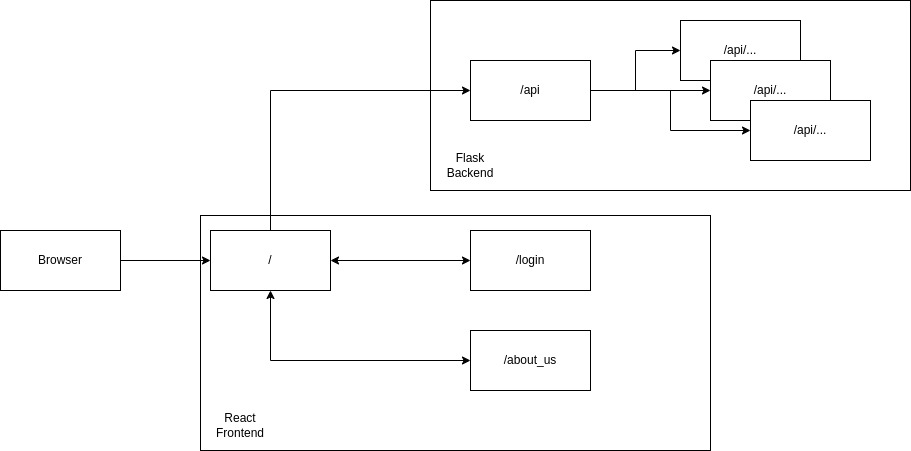
\includegraphics[width=\textwidth]{../images/navigation tree}
    \caption{Navigation tree for single-page React application with Flask backend}
    \label{fig:navigationTree}
\end{figure}

The navigation tree for this application is as shown in~\ref{fig:navigationTree}.

Deciding between a single-page application (SPA) versus a multi-page application (MPA) came down to multiple concerns such as user experience and use case.
SPAs allow the user to interact with the application without having to browse through pages for actions such as log-in.


\subsection{Wireframe}\label{subsec:wireframe}

\begin{figure}
    \centering
    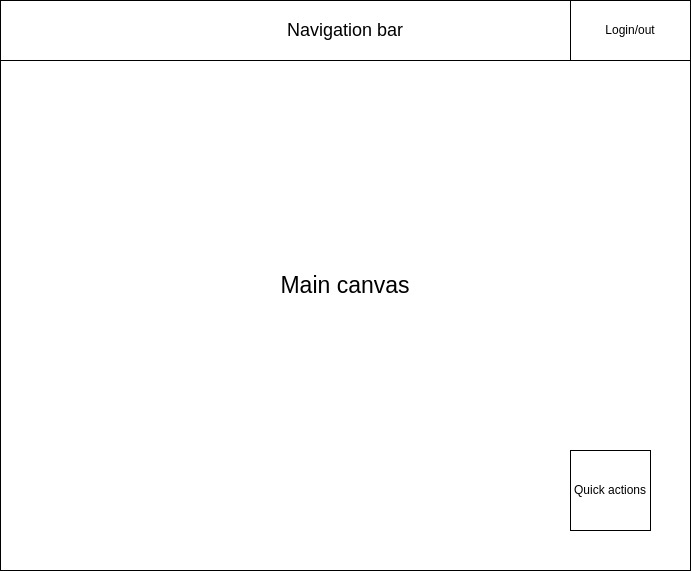
\includegraphics[width=\textwidth]{../images/wireframe}
    \caption{Wireframe for application}
    \label{fig:wireframe}
\end{figure}

